\section{Introduction}
\label{sec:intro}
Motion may be the only way to identify objects in video with low signal-to-noise-ratio (SNR), camouflage, or complex textures that may hinder frame-by-frame object detection. The human visual system is excellent at capturing observable motion~\cite{giese2003neuro}, a capability which has not yet been reproduced by modern computer vision models. Learning to exploit motion cues will improve models' abilities to detect and track objects of interest in noisy video.

In several scientific \cite{Holste2024} and medical applications \cite{sundararajan2018DL4Bio, dargan2020DL4Applications}, clean (noise-free) imagery are not available to train image or video denoisers. One attractive element of self-supervised models is their ability to find the signal within the noisy imagery itself. Self-supervision can, too, be more robust and generalizable to various noise type \cite{shi_how_2022, marks2024closer}.

% Obtaining sufficient annotations to train supervised models in video can be prohibitively expensive, especially for scientific  \cite{Holste2024} or medical \cite{sundararajan2018DL4Bio, dargan2020DL4Applications} applications, and delays the deployment of models when tackling novel signal statistics.
% For example, datasets can be site-specific for ecology or environmental departments, and training a bespoke supervised object detector presents significant resource challenges \TODO{\CITE{}}. 
% Data is limited in medical imaging and biometrics, and obtaining annotations presents significant cost and time delays \cite{sundararajan2018DL4Bio, dargan2020DL4Applications}. 
% Once trained, supervised detectors may not generalize well and may need additional annotations to be adapted to other locations with different background and foreground distributions\cite{oza2021unsuperviseddomainadaptationobject}, which may require additional supervision \cite{Danish_2024_CVPR}. 
% On the other hand, models trained using self-supervision can be more robust \cite{shi_how_2022, marks2024closer}.
% \TODO{}
% \TODO{\CITE{}} - \MM{ add paper that shows generally unsupervised/ssl pretraining is more robust.}
This work aims to enhance motion signals in low-signal-to-noise (SNR) data with non-stationary backgrounds, such as underwater, ultrasound, and sonar videos, to improve downstream supervised classification, detection, and tracking. We address sensor, background, and noise challenges with \NAME{}, a self-supervised learning method to boost signal in noisy video. We exploit object motion to boost the SNR across frames. Inspired by work on self-supervised reconstruction \cite{khalil2024learning, sun2022bkind}, self-supervised video understanding \cite{recasens2021broaden}, and anomaly detection  \cite{yang2023anom, liu2018anom}, we use an encoder to encode appearance frames, a temporal bottleneck, and a decoder network to reconstruct the denoised frame. 
%Our method enables the model to denoise based on spatiotemporal reconstruction similarity.

% Figure 1
\begin{figure}[tp]
    \centering
    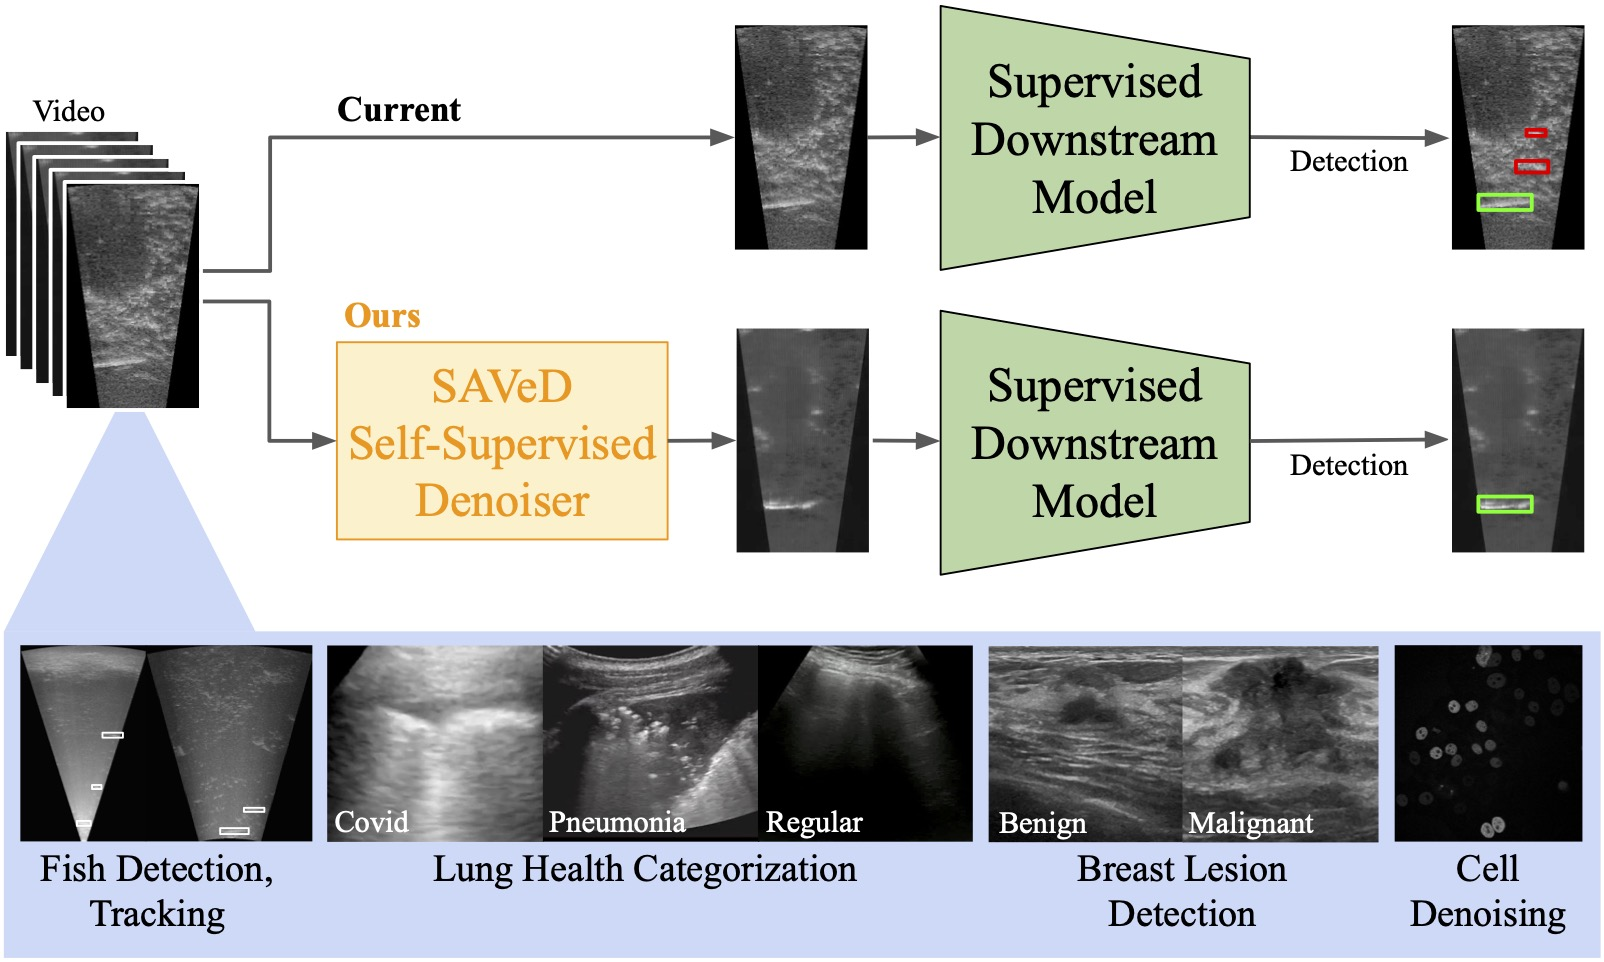
\includegraphics[width=\linewidth]{figs/teaser.jpg}
    \caption{\textbf{SpatioTemporal Denoising improves classification, detection, tracking, and counting in video.} 
    We denoise sonar and ultrasound videos of fish in a river, lung scans, breast lesion scans, and cell microscopy to improve downstream classification, detection, tracking, and counting tasks. 
    We propose a self-supervised method to enhance the foreground signal of video frames without manual annotations or clean imagery. 
    Our method works on grayscale videos with: non-stationary backgrounds, low signal-to-noise-ratios, and a variable number of objects in a video.}
    \label{fig:fig1}
\end{figure}

% Unsupervised and self-supervised methods are increasingly used for object localization and action recognition \cite{khalil2024learning, sun2022bkind, dave2022tclr, tong2022videomae, schiappa2023sslvsurvey, sun2023mabe22}. 
% However, existing methods do not address low-SNR videos.
% %with an undefined number of objects of interest \CITE{}. 
% Furthermore, while some methods \cite{engilber2023multi, feng2025multiview} handle changes in camera view-angle, they do not handle cases where the camera is stationary and the background is not.
% make the distance between the three input arrows the same
% align the other arrows/lines with the middle
% make all the font sizes the same 
% align all of the captions and stuff to the same height as video frames
% lower I_t-1 and I_t and align together with the reconstructed one and the target

\noindent Our main contributions are:
\begin{itemize}
    \item We propose \NAME{}, a novel, state-of-the-art, resource-efficient self-supervised method to improve the signal in low-SNR video with variable numbers of agents and non-stationary background; details are in \cref{sec:method}. %Efficiency is expressed as training time. 
    \item We introduce a novel denoising metric, $FBD$, that does not rely on clean imagery; it instead relies on background-foreground appearance distribution differences, in \cref{sec:method}.
    \item We propose a rich benchmark for low-SNR video denoising consisting of a diverse collection of low-SNR video domains (sonar video of fish, ultrasound video of lungs and breast tissue, and microscopy video) and a diverse collection of downstream visual tasks (classification, detection, tracking, and counting), in \cref{sec:experiments}.
\end{itemize}